\textbf{Задачи из ЕГЭ по математике базового уровня тип №16}

	\begin{figure}[h]
		\centering
		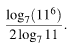
\includegraphics[width=0.11\linewidth]{VM/t1612.png}
		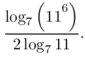
\includegraphics[width=0.11\linewidth]{VM/t1614.png}
		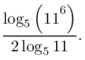
\includegraphics[width=0.11\linewidth]{VM/t1615.png}
		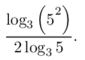
\includegraphics[width=0.11\linewidth]{VM/t1616.png}
		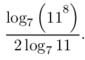
\includegraphics[width=0.11\linewidth]{VM/t1617.png}
		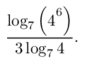
\includegraphics[width=0.11\linewidth]{VM/t1618.png}
\end{figure}
	
\textbf{Шаблон задач}

\lstinputlisting{paragrafs/Zadachi/3}
	
Отличительной особенностью этих шаблонов от предыдущего, является другая библиотека - \texttt{setEvaluationTask}. Помимо самой генерации задачи, на основе переменных их первой части, она так же сама решает сгенерированный пример, и проверяет его ответ. 

Если ответ не является удовлетворительным, а именно таким, что пользователь просто не сможет ввести его на клавиатуре (Ответ представляет из себя бесконечную десятичную дробь, или просто очень длинную), то программа, отслеживает эту ошибку с помощью цикла \texttt{retryWhileError} и предпринимает ещё попытку составить задание с цельным ответом. Количество таких попыток указано внизу кода программы. Если за установленное число попыток, программа так и не получит правильно сгенерированную задачу, то она выведет сообщение об ошибке.

За отображение логарифма на экране здесь отвечает специальная встроенная функция: \texttt{varlog}

\textbf{Сгенерированные по шаблону задачи}

\begin{figure}[h]
		\centering
		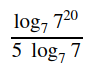
\includegraphics[width=0.11\linewidth]{VM/varlog1.png}
		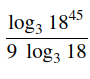
\includegraphics[width=0.11\linewidth]{VM/varlog2.png}
		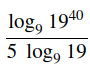
\includegraphics[width=0.11\linewidth]{VM/varlog3.png}
		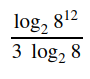
\includegraphics[width=0.11\linewidth]{VM/varlog4.png}
		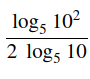
\includegraphics[width=0.11\linewidth]{VM/varlog5.png}
		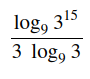
\includegraphics[width=0.11\linewidth]{VM/varlog6.png}
\end{figure}

Также эта библиотека способна сама убирать некоторые скобки, если они не влияют на решение задания, или сама выполнть арифметическую операцию. Но в некотрых случаях, это не является необходимостью. Например как в этой задаче базового типа. Здесь скобки нужны лишь для наглядности, и не оказывают никакого влияния на решение этого примера, но их всё же необходимо сохранить.

\begin{figure}[h]
		\centering
		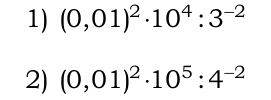
\includegraphics[width=0.4\linewidth]{VM/t1611.png}
		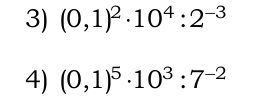
\includegraphics[width=0.4\linewidth]{VM/22.png}
\end{figure}

 Чтобы программа не высчитывала сама то, что стоит оставить, используются следующие команды:
\\ \texttt{forceBrackets} - для сохранение скобок.
\\ \texttt{divideColon} - для вывода знака деления «:».

Шаблон задачи, использующий эти специальные команды

\lstinputlisting{paragrafs/Zadachi/4}

\textbf{Сгенерированные по шаблону задания}

		\begin{figure}[h]
		\centering
		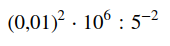
\includegraphics[width=0.35\linewidth]{VM/dv1.png}
		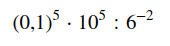
\includegraphics[width=0.35\linewidth]{VM/dv2.png}
		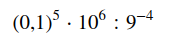
\includegraphics[width=0.35\linewidth]{VM/dv3.png}
		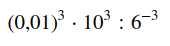
\includegraphics[width=0.35\linewidth]{VM/dv4.png}
\end{figure}

